% !TEX root = sbaconf.tex
%===============================================================================
% $Id: ifacconf.tex 19 2011-10-27 09:32:13Z jpuente $  
% Template for IFAC meeting papers
% Copyright (c) 2007-2008 International Federation of Automatic Control
%===============================================================================
\documentclass[a4paper]{ifacconf}

\usepackage{graphicx,amsmath,url}      % include this line if your document contains figures
\usepackage[round]{natbib}             % required for bibliography
%===============================================================================

% If in Portuguese or Spanish, choose
\def\portugues{1} 
\usepackage[spanish,brazil,english]{babel}
\usepackage[T1]{fontenc}
%\usepackage[utf8]{inputenc}
\usepackage{unicode}
\usepackage{ae}
\usepackage{placeins}
\usepackage{multicol}
\usepackage{multirow}
\usepackage{cuted}
\usepackage{graphicx}
\usepackage{amsmath} % for 'bmatrix' environment
\newcommand\norm[1]{\left\lVert#1\right\rVert}
\newcommand\normx[1]{\left\Vert#1\right\Vert}
\newcommand\Hinfty{\mathcal{H}_\infty}
\newcommand\Hdois{\mathcal{H}_2}
\newcommand\Ldois{\mathcal{L}_2}
\newcommand\ms{290}
\newcommand\mus{40}
\newcommand\bls{700}
\newcommand\bnls{200}
\newcommand\bys{400}
\newcommand\kls{235\cdot10^2}
\newcommand\knls{235\cdot10^4}
\newcommand\kt{190\cdot10^3}
 
\if\portugues1
% =====================================================================
% =====================================================================
% If the manuscript is in Spanish, please change the texts adequatelly.
% You may also add other definitions in this part.
 \newtheorem{teorema}[thm]{{\em Teorema}}{ }
 \newtheorem{lema}[thm]{{\em Lema}}{ }
 \newtheorem{corolario}[thm]{{\em Corolário}}{ }
 \newenvironment{prova}{{\bf Prova.}}{ }
% ===============================================================
\fi

\begin{document}
	
    \selectlanguage{brazil}
	
    \begin{frontmatter}
        
        \title{Síntese de observador e controlador por realimentação de estados para controle de suspensão veicular ativa, não-linear} 

        \author[First]{Charles Quirino Pimenta} 
        
        \address[First]{Programa de Pós-Graduação em Engenharia Elétrica - Universidade Federal de 
Minas Gerais - Av. Antônio Carlos 6627, 31270-901, Belo Horizonte, MG, Brasil\\ e-mail:charlesqp@ufmg.br.}
        
        \selectlanguage{english}
        \renewcommand{\abstractname}{{\bf Abstract:~}}
        \begin{abstract}  Escrever o Abstract em Inglês.
        
        \vskip 1mm% não altere esse espaçamento
        \selectlanguage{brazil}
        {\noindent \bf Resumo}: Escrever o Abstract em português.
        \end{abstract}
        
        \selectlanguage{english}
        
        \begin{keyword} Linear systems; LTI; State feedback control; State Observer; Luenberger Observer; Vehicle active suspension;
        
        \vskip 1mm% não altere esse espaçamento
        \selectlanguage{brazil}
        {\noindent\it Palavras-chaves:} Sistemas lineares; LTI; Controle por realimentação de estados; Observador de estados; Observador de Luenberger; Suspensão ativa veicular;
        \end{keyword}
        
        \selectlanguage{brazil}
        
        \end{frontmatter}

    \section{Introdução}
        \subsection{Métodos de Lyapunov}
A bibliografia de engenharia de controle mostra o uso dos métodos de Lyapunov para a análise e síntese de controladores para sistemas lineares, como pode ser encontrado em \cite{ChenLSTI}. De uma forma geral, utiliza-se controladores lineares baseados nas funções de Lyapunov de forma quadrática. O controlador linear é baseado em modelos linearizados do sistema na proximidade de um ponto de equilíbrio, garantindo a estabilidade local do sistema controlado. Além disso, utilizando controladores é possível garantir a estabilidade do sistema em malha fechada, podendo se associar a qualquer controlador critérios de desempenho, como tempo de acomodação e máximo sobressinal (\cite{Hang1987RefinementsOT}; \cite{601347}; \cite{1049598}), normas $H_2$ (\cite{4789992}) e $H_\infty$ (\cite{Petersen}; \cite{Wang1992RobustCO}), taxa de convergência (\cite{Elia2001StabilizationInformation}; \cite{LORIA200213}), dentre outros.
\subsection{Problema de amortecimento de vibrações em veículos}
Uma suspensão veicular tem a função de isolar os passageiros e o chassi de vibrações originadas das irregularidades da estrada, além disso, atuam para garantir a estabilidade do veiculo durante manobras de condução em pista.
Existem três tipos de suspensão veicular: suspensão passiva, ativa e semiativa. Esta classificação é dada de acordo com a presença e o tipo de controle utilizado para minimizar as vibrações transmitidas ao chassi.
Sistemas de controle passivo são os sistemas de suspensão convencionais, compostos por molas, amortecedores e pneus. O sistema de controle passivo só é capaz de atuar em uma banda de frequência restrita, limitando-se a utilização em sistemas com frequências fora desta banda. Este tipo de sistema proporciona uma viagem menos confortável e estável ao carro em comparação aos sistemas de amortecimento ativo e semiativo. As característica importante deste tipo de sistema é ser caracterizado por não empregar energia externa ao sistema, além de ser o mais barato dentre todos.
Um sistema de suspensão ativa é um sistema capaz de atuar em diferentes bandas de frequência, através da utilização de atuadores, sensores e sistemas eletrônicos de controle. A desvantagem está na elevada quantidade de energia que os componentes utilizados necessitam, demandando o uso de uma fonte de energia externa, isto implica em um produto final de custo mais elevado quando comparado com sistemas de suspensão passiva.
Um sistema de suspensão semiativa também apresenta funcionalidade em diversas bandas de frequência, porém, não possui a obrigatoriedade de uma fonte de tensão externa permanente de grande porte. Outra vantagem deste tipo de sistema é que este, na falta de energia, comporta-se como um sistema passivo, agregando mais confiabilidade e segurança ao veículo. Por fim, um sistema de suspensão semiativa possui custo intermediário entre as demais opções.
O foco deste trabalho recai sobre o sistema de suspensão ativa com um atuador generalizado, apresentando assim a implementação de um controlador ativo aplicado a um sistema de suspensão veicular com modelo não linear.
\subsection{Observadores de estados}
Segundo a definição de \cite{EllisObserver}, um observador é uma estrutura matemática que, a cada instante de tempo t, constrói uma estimativa $\hat{x}(t)$ do estado $x(t)$ através da combinação das medidas das entradas $u(t)$ e saídas $y(t)$, provenientes de sensores. Em aplicações de controle de sistemas, mais especificamente no controle por realimentação de estados, a realimentação envolve a medição de todo o vetor de estado, o que nem sempre é possível ou viável economicamente. A solução neste caso é estimar os estados faltantes a partir das saídas que são possíveis de ser medidas. Desta forma, utiliza-se o vetor de ganhos calculado como se o estado fosse, de fato, medido. Assim, substitui-se o estado pelo estado estimado, multiplicado pelo vetor de ganhos do controlador, para fechar a malha de controle.
O estimador de estados foi chamado de observador por Luenberger em \cite{Luenberger1971AnObservers} e \cite{Luenberger}, o primeiro a apresentar o conceito e por este motivo é chamado de observador de Luenberger. Sua principal característica que o diferencia dos demais é que observador de Luenberger corrige a equação de estimação do estado com uma realimentação do erro de estimação $y(k)-\hat{y}(k)$.
De maneira geral, um problema dos observadores é o fato que perturbações externas corrompem o sinal do estado estimado, pois estas afetam a variável de estado real na planta controlada mas não são incluídas no calculo do preditor. De fato, perturbações não podem ser incluídas no cálculo da predição por que estas são desconhecidas na maioria das vezes. Com poucas excessões, perturbações não são medidas diretamente.  
\subsection{Observadores de Entradas Desconhecidas}
Observadores de Entradas Desconhecidas (do inglês,Unknown Input Observers, UIOs) são uma classe de observadores que possui como característica a possibilidade de desacoplar as entradas desconhecidas (erros de modelagem,distúrbios, perturbações, dentre outros) do erro de estimação. Um UIO trata o problema da corrupção do estado estimado, podendo ser aplicados para o projeto de controladores baseados em observadores (\cite{Zasadzinski1995LoopTR}), sendo que o UIO sintetizado é empregado para estimar os estados do sistema, os quais são posteriormente utilizados para realizar o controle por realimentação de estados. Outra aplicação para controle existente na literatura surge do uso de UIOs para estimativa de entradas desconhecidas (distúrbios)utilizada em aplicações como Disturbance Accommodation Control(DAC) (\cite{Chen2016Disturbance-Observer-BasedOverview}).
    \section{Objetivos}
        Tendo em vista o problema de projetar controladores para sistemas de suspensão veicular ativa com o objetivo de melhorar o conforto e a segurança na condução do veiculo. Este trabalho tem como objetivo principal analisar o efeito do uso de observadores de entradas desconhecidas na síntese de um sistema de controle por realimentação de estados baseado em observador para um sistema de suspensão veicular, linear, invariante no tempo com dependência paramétrica e incertezas politópicas.  
A principal motivação deste trabalho é projetar observadores e controladores com estruturas simples, capazes de atenderem aos requisitos de projeto e que não necessitem mensurar ou estimar os parâmetros do sistema. Comparar o desempenho entre dois sistemas de controle empregando dois tipos diferentes de observador de estados. Em ambos os sistemas de controle será empregado o mesmo controlador de realimentação de estados, que será sintetizado por meio da técnica de \( \mathcal{D}\)-alocação de polos via LMIs, garantindo assim estabilidade assintótica para os sistemas projetados.
Para alcançar o objetivo principal, os seguintes objetivos específicos foram propostos:
\begin{itemize}
    \item Realizar a modelagem matemática de um sistema de suspensão não linear de um quarto de veículo com dois graus de liberdade.
    \item Realizar a linearização do modelo completo proposto.
    \item Projetar um observador de Luenberger para a estimação das variáveis de estados necessárias para o funcionamento da estratégia de controle.
    \item Projetar um controlador linear por realimentação de estados com ganho constante por meio da aplicação da técnica de \( \mathcal{D}\)-alocação de polos via desigualdades matriciais lineares (LMIs). Uma \( \mathcal{D}\)-Região é proposta para garantir a estabilidade e os requisitos de desempenho de tempo de acomodação e máxima sobrelevação percentual mesmo sob condições de incerteza dos parâmetros do sistema.
    \item Projetar um observador de entradas desconhecidas, pelo método das desigualdades matriciais lineares (LMIs), para a estimação das variáveis de estados necessárias para o funcionamento da estratégia de controle.
    \item Realizar simulações temporais com o controlador proposto para o sistema linearizado empregando as diferentes metodologias de observadores e comparar os resultados.
\end{itemize}
    \section{Revisão Bibliográfica}
        \subsection{Modelo matemático do sistema de suspensão não linear para um quarto de veículo }
O modelo de um quarto de carro consiste em isolar uma quarta parte do veículo e estudar isoladamente o comportamento do sistema de suspensão para esta seção. Para veículos com peso igualmente distribuído, os resultados são muito próximos ao do modelo completo. Geralmente os modelos para um quarto de carro tem 2 graus de liberdade, sendo estes o deslocamento vertical da massa suspensa e da massa não suspensa, o que pode ser observado na figura \ref{fig:massa_mola_nao_linear_controlavel} a seguir. Este modelo é composto por uma massa suspensa que representa a carroceria do veículo e uma massa não suspensa que representa o conjunto eixo e roda. Estas massas são conectadas pela mola e pelo amortecedor. O contato do veículo com a pista de rolamento é realizado através do pneu. O sistema é exitado, ou perturbado, pelas irregularidades da pista.
\FloatBarrier
\begin{figure}[htbp]
  \begin{centering}
    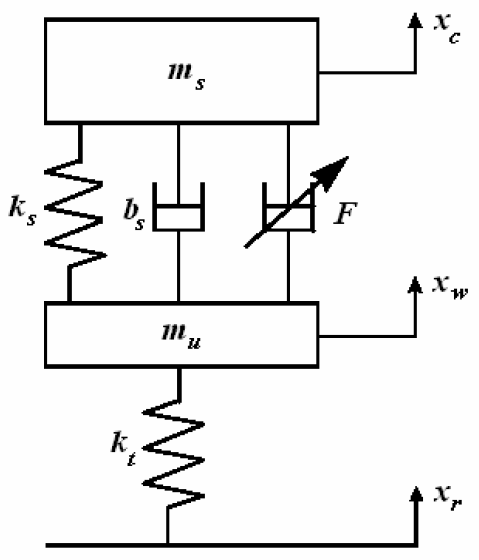
\includegraphics[width=7cm,height=5.25cm]{img/massa_mola_nao_linear_controlavel.png}
    \caption{Modelo de suspensão para um quarto de carro.} 
    \label{fig:massa_mola_nao_linear_controlavel}
  \end{centering}
\end{figure}
\FloatBarrier
Na figura \ref{fig:massa_mola_nao_linear_controlavel}, $m_s$ representa a massa suspensa que consiste em um quarto da massa total da carroceria do veículo em \emph{kg}, $m_u$ representa a massa não suspensa ou a massa do eixo e da roda em \emph{kg}, $b_s$ representa o coeficiente de amortecimento do amortecedor passivo em \emph{Ns/m}, $k_s$ representa o coeficiente de elasticidade do feixe de molas da suspensão, segundo a lei de Hooke, em \emph{N/m}, $k_t$ representa o coeficiente de elasticidade do pneu, segundo a lei de Hooke, em \emph{N/m}, $x_r$ representa o deslocamento vertical da pista, onde o sufixo $r$ significa \emph{road}, em \emph{m}, $x_w$ representa o deslocamento vertical da roda, onde o sufixo $w$ significa \emph{wheel}, em \emph{m} e $x_c$ representa o deslocamento vertical da carroceria, onde o sufixo $c$ significa \emph{carr}, em \emph{m}. Na mesma figura o simbolo $F$ representa a atuação de um dispositivo amortecedor com características dinâmicas, seja ele ativo ou semi-ativo, em \emph{N}.
  
O diagrama de corpo livre do sistema pode ser construído tomando-se como referencia a coordenada da posição do eixo da roda $x_w$ como pode ser observado nas figuras \ref{fig:corpo_livre_ms} e \ref{fig:corpo_livre_mu} a seguir:
\FloatBarrier
\begin{figure}[htbp]
    \begin{centering}
      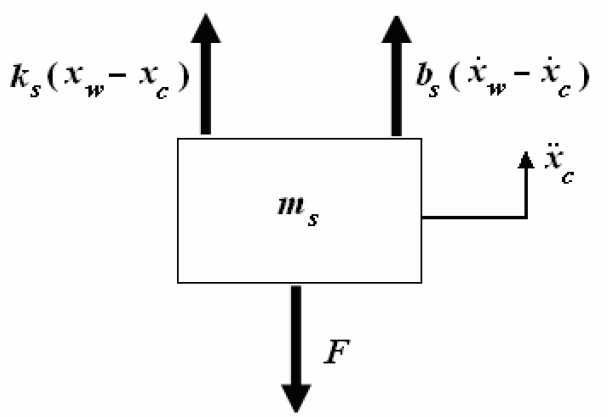
\includegraphics[width=7cm,height=5.25cm]{img/corpo_livre_ms.png}
      \caption{Diagrama de corpo livre para a massa $m_s$.} 
      \label{fig:corpo_livre_ms}
    \end{centering}
\end{figure}
\FloatBarrier
\begin{figure}[htbp]
  \begin{centering}
    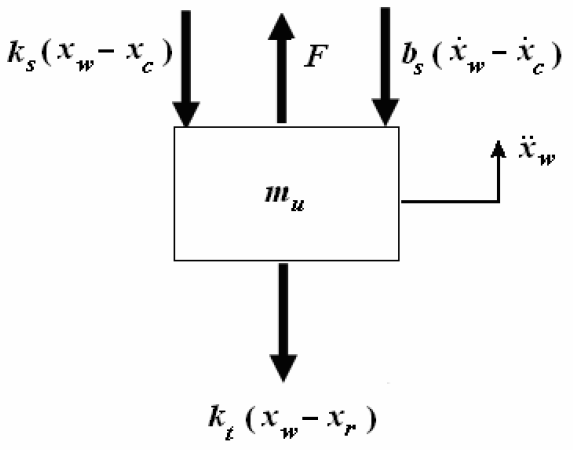
\includegraphics[width=7cm,height=5.25cm]{img/corpo_livre_mu.png}
    \caption{Diagrama de corpo livre para a massa $m_u$.} 
    \label{fig:corpo_livre_mu}
  \end{centering}
\end{figure}
\FloatBarrier
  
Aplicando a segunda lei de Newton $\sum{F}=m.a$, a cada uma das massas separadamente, o sistema para o modelo de um quarto de carro da figura \ref{fig:massa_mola_nao_linear_controlavel} pode ser representado pela seguinte equação:
  
\begin{equation} \label{eq:massa_mola_linear}
  \begin{split}
    m_{s} \ddot{x}_{c} =& b_{s}(\dot{x}_{w}-\dot{x}_{c}) + k_{s}(x_{w}-x_{c}) - F\ \\
    m_{u} \ddot{x}_{w} =& -b_{s}(\dot{x}_{w}-\dot{x}_{c}) - k_{s}(x_{w}-x_{c})+k_{t}(x_{w}-x_{r}) + F
  \end{split}
\end{equation}
  
A equação \eqref{eq:massa_mola_linear} representa o modelo do sistema na forma linear. Porém a mola $k_s$, o amortecedor $b_s$ e o amortecedor dinâmico ativo podem ser modelados através de modelos lineares ou modelos não lineares. \\
Uma mola linear obedece a lei de Hooke apresentando uma deformação proporcional ao carregamento. Em uma mola não linear o coeficiente de elasticidade da mola cresce exponencialmente conforme se afasta do ponto de equilíbrio estático.
Para um modelo de mola não linear, podemos utilizar seguinte expressão para a força da mola $ k_{s}(x_{w}-x_{c})$:
  
\begin{equation} \label{eq:mola_nao_linear}
  k_{s}(x_{w}-x_{c}) = k^{l}_{s}(x_{w}-x_{c})+k^{nl}_{s}(x_{w}-x_{c})^{3}
\end{equation}
    
Na equação \eqref{eq:mola_nao_linear} o coeficiente $k^{l}_{s}$ representa o coeficiente de elasticidade do termo da faixa de operação linear e o coeficiente $k^{nl}_{s}$] representa o coeficiente de elasticidade do termo da faixa de operação não linear do feixe de molas em uma situação real.\\
A não linearidade do amortecedor permite que pequenos movimentos causados pelo perfil da estrada gerem apenas um pequeno impacto na carroceria além de apresentar saturação e histerese. Para um modelo de amortecedor não linear, podemos utilizar a seguinte expressão:
 
\begin{equation} \label{eq:amortecedor_nao_linear}
  \begin{aligned}
    b_{s}(\dot{x}_{w}-\dot{x}_{c}) =\ \ &b^{l}_{s}(\dot{x}_{w}-\dot{x}_{c}) - b^{y}_{s}\mid\dot{x}_{w}-\dot{x}_{c}\mid \\
    + &b^{nl}_{s}\sqrt{\mid\dot{x}_{w}-\dot{x}_{c}\mid}sgn(\dot{x}_{w}-\dot{x}_{c}) 
  \end{aligned}
\end{equation}
  
Na equação \eqref{eq:amortecedor_nao_linear} o coeficiente $b^{l}_{s}$ representa o coeficiente de amortecimento do termo da faixa de operação linear, o coeficiente $b^{l}_{s}$ representa o coeficiente de amortecimento do termo da faixa de operação não linear e o coeficiente $b^{y}_{s}$ representa a característica de comportamento assimétrico do amortecedor.
  
Substituindo as equações \eqref{eq:mola_nao_linear} e \eqref{eq:amortecedor_nao_linear} em \eqref{eq:massa_mola_linear}, obtemos as seguintes equações diferenciais dinâmicas de segunda ordem que, representam a dinâmica de um sistema de suspensão ativa não linear:
  
\begin{equation} \label{eq:massa_mola_nao_linear}
  \begin{aligned}
     m_{s} \ddot{x}_{c} =\ \ &k^{l}_{s}(x_{w}-x_{c})+k^{nl}_{s}(x_{w}-x_{c})^{3}+b^{l}_{s}(\dot{x}_{w}-\dot{x}_{c})\\
              -&b^{y}_{s}\mid\dot{x}_{w}-\dot{x}_{c}\mid+b^{nl}_{s}\sqrt{\mid\dot{x}_{w}-\dot{x}_{c}\mid}sgn(\dot{x}_{w}-\dot{x}_{c})\\ 
              -&F\\
     m_{u} \ddot{x}_{w} = -&k^{l}_{s}(x_{w}-x_{c})-k^{nl}_{s}(x_{w}-x_{c})^{3}-b^{l}_{s}(\dot{x}_{w}-\dot{x}_{c})\\ 
              +&b^{y}_{s}\mid\dot{x}_{w}-\dot{x}_{c}\mid-b^{nl}_{s}\sqrt{\mid\dot{x}_{w}-\dot{x}_{c}\mid}sgn(\dot{x}_{w}-\dot{x}_{c})\\
              -&k_{t}(x_{w}-x_{r})+F\\
  \end{aligned}
\end{equation}
    
\subsection{Modelo Não Linear de um sistema de suspensão semi-ativa, não linear, de um quarto de veículo, com dois graus de liberdade }
Realizando a distributiva no sistema descrito em \eqref{eq:massa_mola_nao_linear} e propondo as seguintes substituições para as variáveis de estado das equações e reorganizando os termos, obtemos: 
\begin{equation*}
  \begin{split}
    x_{1}=&x_{c};\ \ \\
    x_{2}=&\dot{x}_{c};\ \ \\ 
    x_{3}=&x_{w};\ \ \\        
    x_{4}=&\dot{x}_{w};\ \ \\
  \end{split}
  \begin{split}
    \dot{x}_{1}=&\dot{x}_{c};\ \ \\
    \dot{x}_{2}=&\ddot{x}_{c};\ \ \\
    \dot{x}_{3}=&\dot{x}_{w};\ \ \\    
    \dot{x}_{4}=&\ddot{x}_{w};\ \ \\
  \end{split}
  \begin{split}
    w=&x_{r};\ \ \\
    u=&F;\ \ \\
  \end{split} 
\end{equation*}
\begin{equation} \label{eq:massa_mola_nao_linear_SS}
  \begin{aligned}
    \dot{x}_{1}=&\ \ \ \ x_{2}\\    
    \dot{x}_{2}=&-\frac{k^l_s}{m_s}x_1-\frac{b^l_s}{m_s}x_2+\frac{k^l_s}{m_s}x_3+\frac{b^l_s}{m_s}x_4-\frac{k^{nl}_s}{m_s}(x_3-x_1)^3\\
          &+\frac{b^y_s}{m_s}\mid x_4-x_2\mid+\frac{b^{nl}_s}{m_s}\sqrt{\mid x_4-x_2\mid}sgn(x_4-x_2)\\
          &-\frac{1}{m_s}u\\  
    \dot{x}_{3}=&\ \ \ \ x_{4}\\
    \dot{x}_{4}=&\ \ \ \ \frac{k^l_s}{m_u}x_1+\frac{b^l_s}{m_u}x_2-\frac{k^l_s}{m_u}x_3-\frac{b^l_s}{m_u}x_4+\frac{k^{nl}_s}{m_u}(x_3-x_1)^3\\
          &-\frac{b^y_s}{m_u}\mid x_4-x_2\mid-\frac{b^{nl}_s}{m_u}\sqrt{\mid x_4-x_2\mid}sgn(x_4-x_2)\\
          &+\frac{k_t}{m_u}w+\frac{1}{m_u}u\\
  \end{aligned}
\end{equation}
  
\subsection{Linearização do modelo em espaço de estados}

O sistema proposto possui um ponto de equilíbrio na origem do sistema formado pelas variáveis de estado:
\begin{equation*}
    \begin{split}
        x_1=\ \ &0\\
        x_2=\ \ &0\\
        x_3=\ \ &0\\
        x_4=\ \ &0\\
    \end{split}
\end{equation*}
Para realizar a linearização em torno do ponto de operação escolhido calcula-se a Jacobiana do sistema de equações dinâmicas não lineares descrito em \eqref{eq:massa_mola_nao_linear}. Em seguida, calcula-se o valor da Jacobiana no valor específico do ponto de equilibro, assim obtemos as matrizes $A$ e $B$ do sistema linearizado exibidas a seguir:
 
\begin{equation}\label{ed:linsys:ax}
    \begin{split}
        \mathbf{A} =
        \begin{bmatrix}
            0 & 1 & 0 & 0 & \\            
            -\frac{k_{s}^{l}}{m_s}&-\frac{b_{s}^{l}}{m_s}&\frac{k_{s}^{l}}{m_s}&\frac{b_{s}^{l}}{m_s} &\\ \  
            0 & 0 & 0 & 1 & \\
            \frac{k_{s}^{l}}{m_u}&\frac{b_{s}^{l}}{m_u}&-\frac{(k_{s}^{l}+k_t)}{m_u}&-\frac{b_{s}^{l}}{m_u} &\\
        \end{bmatrix};
    \end{split}
    \begin{split}
       \mathbf{x} = 
        \begin{bmatrix}
             x_1 &\\
             x_2 &\\
             x_3 &\\
             x_4 &\\
        \end{bmatrix}; 
    \end{split}
\end{equation}
    
\begin{equation} \label{ed:linsys:BuBw}
    \begin{split}
        \mathbf{B_u} = 
        \begin{bmatrix}
            0 & \\            
            -\frac{1}{m_s}&\\ \\  
            0 & \\
            \frac{1}{m_u}&\\
        \end{bmatrix};
    \end{split}
    \begin{split}
        \mathbf{B_w} = 
        \begin{bmatrix}
            0 & \\            
            0 &\\ \\  
            0 & \\
            \frac{k_t}{m_u}& \\
        \end{bmatrix}
    \end{split}
\end{equation}
    
É esperado que o  sistema linearizado se aproxime do sistema não linear enquanto opera na vizinhança do ponto de equilíbrio utilizado para linearização. 
   
\subsection{Especificações da Resposta Transitória para Sistemas Subamortecidos}
As características de um sistema de controle são geralmente especificadas em termos da resposta transitória para uma entrada em degrau. Para sistemas LTI, quando a resposta ao degrau é conhecida, pode-se calcular a resposta a qualquer tipo de entrada e costuma-se utilizar condição inicial de sistema em repouso. 
Considere uma função de transferência de 2\textdegree ordem do tipo:

\begin{equation} \label{eq:2ordmdl}
  G(s) = \frac{\omega^2_n}{s^2+2\xi \omega_ns +\omega^2_n}
\end{equation}

Que é o modelo da função de transferência desejada em malha 
fechada no modelo SISO. O modelo \eqref{eq:2ordmdl} define uma função de transferência estável e desejada, em que $\omega_n$ e a frequência natural e $\xi$ é o coeficiente de amortecimento.
As seguintes especificações são as mais utilizadas para obtenção de $\omega_n$ e de $\xi$ :

\begin{equation} \label{eq:wnxi}
  \begin{split} 
    \xi=-\frac{ln\left( M_O \right)}{\sqrt{\pi^2+ln^2(M_O)}}\\
    \omega_n=-\frac{ln\left( 0.02*\sqrt{1-\xi} \right)}{T_{S_{2\%}}*\xi} 
  \end{split}
\end{equation}
  
Onde $MO$ é o máximo overshoot, valor máximo de pico da curva de resposta, medido a partir da unidade. Se o valor da resposta em regime diferir da unidade, utiliza-se a porcentagem máxima de sobressinal (ou ultrapassagem percentual, U.P.) e $t_s$ é o Tempo de acomodação ou assentamento, tempo necessário para que a resposta permaneça com valores no interior de uma certa faixa (usualmente $\pm2\%$ ou $\pm5\%$) em torno do valor final.

A equação \eqref{eq:wnxi} define os parâmetros que serão utilizados para construir os  autovalores do sistema desejado em \eqref{eq:2ordmdl}, tal que $s_{1,2}=-\sigma _p \pm j\omega _d$, sendo que $\sigma _p = \wi\omega _n$ e $\omega _{d}=\omega _{n} \sqrt{1-\xi}$ 
 
\subsection{Observador de Luenberger}\label{sc:luemberger}
Segundo a definição de \cite{EllisObserver}, um observador é uma estrutura matemática que, a cada instante de tempo t, constrói uma estimativa $\hat{x}(t)$ do estado $x(t)$ através da combinação das medidas das entradas $u(t)$ e saídas $y(t)$, provenientes de sensores. Em aplicações de controle de sistemas, mais especificamente no controle por realimentação de estados, a realimentação envolve a medição de todo o vetor de estado, o que nem sempre é possível ou viável economicamente. A solução neste caso é estimar os estados faltantes a partir das saídas que são possíveis de ser medidas. Desta forma, utiliza-se o vetor de ganhos calculado como se o estado fosse, de fato, medido. Assim, substitui-se o estado pelo estado estimado, multiplicado pelo vetor de ganhos do controlador, para fechar a malha de controle.
O estimador de estados foi chamado de observador por Luenberger em \cite{Luenberger1971AnObservers} e \cite{Luenberger}, o primeiro a apresentar o conceito e por este motivo é chamado de observador de Luenberger. Sua principal característica que o diferencia dos demais é que observador de Luenberger corrige a equação de estimação do estado com uma realimentação do erro de estimação $y(k)-\hat{y}(k)$.
De maneira geral, um problema dos observadores é o fato que perturbações externas corrompem o sinal do estado estimado, pois estas afetam a variável de estado real na planta controlada mas não são incluídas no calculo do preditor. De fato, perturbações não podem ser incluídas no cálculo da predição por que estas são desconhecidas na maioria das vezes. Com poucas excessões, perturbações não são medidas diretamente.
Considere o sistema linear e invariante no tempo representado a seguir pela equação \eqref{eq:linsys}:

\begin{equation}\label{eq:linsys}
  \begin{split}
    \dot{x}(t)=&Ax(t)+B_uu(t)+B_ww(t)\\
       y(t)=&Cx(t)+D_uu(t)+D_ww(t)
  \end{split}
\end{equation}

Considere também o observador de estados linear de Luenberger representado a seguir pela equação \eqref{eq:linLue}: 

\begin{equation}\label{eq:linLue}
  \begin{split}
    \hat{\dot{x}}(t)=&(A-LC)\hat{x}(t) + Ly(t) 
  \end{split}
\end{equation}

Onde $x \in \Re^{n_{x} \times 1}$ é o vetor de estados do sistema, $u \in \Re^{n_{u} \times 1}$ é o vetor de entrada de controle, $w \in \Re^{n_{w} \times 1}$ é o vetor de entrada de perturbação, $A \in \Re^{n_{x} \times n_{x}}$, $B \in \Re^{n_{x} \times 1}$, $C \in \Re^{n_{y} \times n_{x}}$, $D_u \in \Re^{1 \times 1}$ e $D_w \in \Re^{1 \times 1}$ são as matrizes do sistema, $y \in \Re^{{n_{y} \times 1}}$ é o vetor de saídas, $z \in \Re^{n_{x} \times 1}$ é o vetor de estados preditos, e $L\in \Re^{n_{x} \times 1}$ é o vetor de ganhos do observador.

Considere o par $(A,C)$ completamente observável. O que implica que a matriz de observabilidade:

\begin{equation}\label{eq:Matrix:MO}
  \mathbb{M_O}=
  \begin{bmatrix}
    C^'&A^'C^'&(A^')^2C^'&\dots&(A^')^{n-1}C^'\\
  \end{bmatrix}    
\end{equation}

Possui $rank(\mathbb{M_O}) = n$
 
Se o par $(A,C)$ for completamente observável é possível encontrar um vetor de ganhos $L\in \Re^{n_{x} \times 1}$ que faça com que o conjunto de autovalores de $A-L*C$ corresponda ao conjunto de autovalores de qualquer matriz $F \in \Re^{n_{x} \times n_{x}}$ arbitrariamente escolhida. 
Definindo-se o erro de estimação de estado como $e=x-\hat(x)$, $L$ deve ser escolhido de maneira que leve $(A-LC)$ à estabilidade rapidamente e sem grandes oscilações), ou seja, L deve fazer com que o erro de observação e,
qualquer que seja o erro inicial, convirja para zero o mais rapidamente possível. Para isso, é muito importante que o observador seja mais rápido 
que o sistema que ele observa, assim ele não introduz erros significativos na dinâmica do sistema controlado. A escolha conveniente dos autovalores de $(A-LC)$ faz com que o erro $e\rightarrow0$ assintoticamente. 
O conjunto de autovalores de $(A-LC)$ pode ser escolhida pela resolução da equação de Lyapunov.
  
\begin{enumerate}
  \item Define-se uma matriz $F \in \Re^{n_{x} \times n_{x}}$ com os autovalores desejados, pelo menos 3 vezes mais rápidos do que o autovalor mais rápido do sistema.
  \item Escolhe-se uma matriz $\bar{k}$ arbitrário tal que $(F,\bar{k})$ seja observável.
  \item {Obtém-se a solução única $T$ da equação de Lyapunov
  \begin{equation} \label{eq:lyapunov}
      A^'T-TF=C^'\bar{k}
  \end{equation}}
  \item {Computa-se o ganho de realimentação:
  \begin{equation} \label{eq:ganho}
      L=\bar{k}T^{-1}
  \end{equation}}
\end{enumerate} 

A implementação do observador de Luenberger em ambiente Simulink é exibida na figura \ref{fig:luemberger_simulink} a seguir:

\FloatBarrier
\begin{figure}[htbp]
  \begin{centering}
    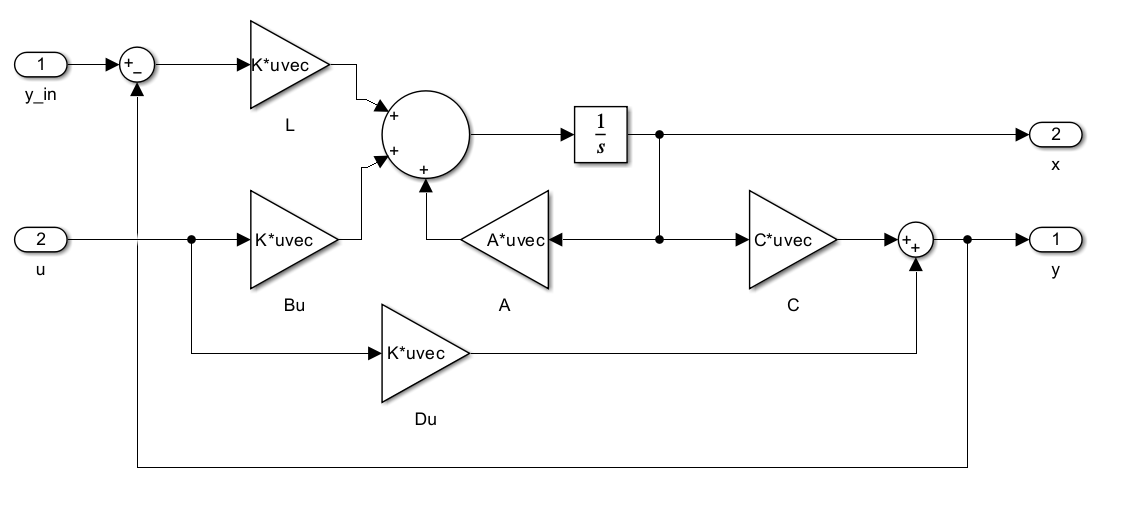
\includegraphics[width=8cm]{img/luenberger_simulink.png}
    \caption{Observador de Luenberger em ambiente Simulink.} 
    \label{fig:luemberger_simulink}
  \end{centering}
\end{figure}
\FloatBarrier

\subsection{Métodos de Lyapunov}
A bibliografia de engenharia de controle mostra o uso dos métodos de Lyapunov para a análise e síntese de controladores para sistemas lineares, como pode ser encontrado em \cite{ChenLSTI}. De uma forma geral, utiliza-se controladores lineares baseados nas funções de Lyapunov de forma quadrática. O controlador linear é baseado em modelos linearizados do sistema na proximidade de um ponto de equilíbrio, garantindo a estabilidade local do sistema controlado. Além disso, utilizando controladores é possível garantir a estabilidade do sistema em malha fechada, podendo se associar a qualquer controlador critérios de desempenho, como tempo de acomodação e máximo sobressinal (\cite{Hang1987RefinementsOT}; \cite{601347}; \cite{1049598}), normas $\Hdois$ (\cite{4789992}) e $\Hinfty$ (\cite{Petersen}; \cite{Wang1992RobustCO}), taxa de convergência (\cite{Elia2001StabilizationInformation}; \cite{LORIA200213}), dentre outros.

\subsection{Desigualdades Matriciais Lineares aplicadas na teoria de controle}
A História do uso de desigualdades matriciais lineares (LMIs) na análise de sistemas dinâmicos tem início nos primeiros anos do século XX, segundo \cite{Boyd1994LinearTheory}, quando \cite{Lyapunov1992TheMotion} publicou seu trabalho sobre o problema geral da estabilidade do movimento. Lyapunov demonstrou que a equação diferencial:
\begin{equation} \label{eq:lyapunovdif}
  \frac{\partial x(t)}{\partial t} = Ax(t), 
\end{equation}
é estável se e somente se existir uma matriz P, definida positiva, tal que:
\begin{equation} \label{eq:lyapunovlmi}
  A^{T}P + PA < 0,
\end{equation}
    
O requisito $P>0, A^{T} P + PA < 0$ é o que chamamos de desigualdade de Lyapunov em P, que é uma LMI. \cite{Lyapunov1992TheMotion} demonstrou que esta LMI pode ser resolvida analiticamente através de um sistema de equações lineares.
    
A teoria de \cite{Lyapunov1992TheMotion} tornou-se conhecida da comunidade de engenharia de controle por volta da década de 1960, com o desenvolvimento do conceito de controle moderno. Porém, segundo \cite{Rodrigues2018ParameterizedSystems}, foi o surgimento dos métodos dos pontos interiores para solução de problemas de programação linear e convexa na década de 1980 que tornou possível que uma enorme variedade de problemas na teoria de controle e sistemas pudessem ser resolvidos de maneira eficiente por meio de métodos numéricos empregando os métodos de Lyapunov.

Segundo \cite{Boyd1994LinearTheory} Uma LMI é descrita pela seguinte expressão:

\begin{equation}\label{eq:defLMI}
  F(x) = F_0 + \sum^{m}_{k=1}X_iF_i, \geq 0
\end{equation}

Onde $x \in \Re^{m}$ F(x) e uma função afim, em que $F_i \in \Re^{n \times m}$, $i = 0, \dots, m$ são matrizes simétricas semi-definidas positivas. Umas das suas características e apresentar o formato simétrico em suas matrizes. A restrição em (12) consiste numa restrição convexa, isto é, o conjunto $x/F(x)\geq 0$ e convexo.
    
\subsection{Observadores de entradas desconhecidas para sistemas LPV}
Baseado nos trabalhos de \cite{SilvaSinteseEstados} e \cite{Dias2022ItaloDias}, Observadores de Entradas Desconhecidas (do inglês,Unknown Input Observers, UIOs) são uma classe de observadores que possuem como característica principal a possibilidade de desacoplar as entradas desconhecidas (erros de modelagem,distúrbios, perturbações, dentre outros) do erro de estimação. Um UIO trata o problema da corrupção do estado estimado, podendo ser aplicados para o projeto de controladores baseados em observadores (\cite{Zasadzinski1995LoopTR}), sendo que o UIO sintetizado é empregado para estimar os estados do sistema, os quais são posteriormente utilizados para realizar o controle por realimentação de estados. Outra aplicação para controle existente na literatura surge do uso de UIOs para estimativa de entradas desconhecidas (distúrbios)utilizada em aplicações como Disturbance Accommodation Control(DAC) (\cite{Chen2016Disturbance-Observer-BasedOverview}).

Do trabalho de \cite{Dias2022ItaloDias}, seja um sistema linear com dependência paramétrica no tempo contínuo dado por:

\begin{equation}\label{eq:part_linsys}
  \begin{split}
    \dot{x}(t)=&A(\alpha)x+B_uu+B_w(\alpha)w\\
       y(t)=&Cx
  \end{split}
\end{equation}

Onde $x \in \Re^{n_{x} \times 1}$ é o vetor de estados do sistema, $u \in \Re^{n_{u} \times 1}$ é o vetor de entrada de controle, $w \in \Re^{n_{w} \times 1}$ é o vetor de entrada de perturbação no sistema e erros de modelagem. $y \in \Re^{n_{y} \times 1}$ é o vetor de saídas mensuráveis e $\alpha \in \Lambda_N$ é o vetor de parâmetros incertos ou variantes no tempo. As matrizes $A$, $B_u$, $B_w$ e $C$ possuem dimensões compatíveis.
O objetivo é projetar um observador de estados na forma:

\begin{equation}\label{eq:UIO}
  \begin{split}
    \dot{h}=&A_hh+B_hu+Ly\\
       \hat{x}=&h-Ey
  \end{split}
\end{equation}

Que seja capaz de rejeitar a entrada desconhecida $w$, com $\hat{x} \in \Re^{n*1}$ definido como o vetor de estados estimados do sistema e $h \in \Re^{n*1}$ definido como o vetor de estados internos do observador. As matrizes $A_h$, $B_h$, L e E são constantes e projetadas para minimizar o erro de estimação dos estados do sistema.

Escolhida a estrutura do observador, define-se o erro de estimação com $e=x-\hat{x}$ e o reescrevemos da seguinte maneira:

\begin{equation}
  e=x-h+E_y = (I+EC)x-h
\end{equation}

Definindo-e a variável de linearização $M=I+EC$, a dinâmica do erro de estimação pode ser reescrita como segue:

\begin{equation} \footnotesize
  \begin{split}
    \dot{e}=&M\dot{x}-\dot{h}\\
    \dot{e}=&M(A(\alpha)x+B_uu+B_w(\alpha)w)-A_hh-B_hu-Ly\\
    \dot{e}=&M(A(\alpha)x+B_uu+B_w(\alpha)w)-A_hh-B_hu-LCx\\
    \dot{e}=&MA(\alpha)x+MB_uu+MB_w(\alpha)w-A_hMx+A_he-B_hu-LCx\\
  \end{split}  
\end{equation}
\normalsize
Que produz o seguinte resultado:

\begin{equation} \footnotesize
  \dot{e}=A_he+(MA(\alpha)-LC-A_hM)x+(MB_u-B_h)u+MB_w(\alpha)w
\end{equation}

O objetivo do observador de entradas desconhecidas é desacoplar os efeitos destas entradas, sejam elas conhecidas ou não, da dinâmica do observador. Para que isto ocorra, as seguintes relações devem ser verdadeiras:

\begin{equation} \label{eq:cond1UIO}
  MB_u-B_h=0  
\end{equation}

\begin{equation} \label{eq:cond2UIO}
  MB_w(\alpha)=0
\end{equation}

\begin{lema}[Condição necessária de existência do UIO] \label{eq:lema1UIO}
  \begin{equation} 
    rank(B_w(\alpha))=rank(CB_w(\alpha)), \forall\alpha \in \Lambda_N
  \end{equation}  
\end{lema}

Desde que todas as condições dadas nas equações \eqref{eq:cond1UIO}, \eqref{eq:cond2UIO} e no Lema \eqref{eq:lema1UIO} sejam atendidas, a dinâmica do erro de estimação é dada por:

\begin{equation} \label{eq:erroUIO}
  \dot{e}=A_he+(MA(\alpha)-LC-A_hM)x
\end{equation}

Ao analisar a Equação \eqref{eq:erroUIO} é possível notar que existe interferência da dinâmica dos estados do sistema \eqref{eq:part_linsys} na dinâmica do erro de estimação. Porém, dado que a matriz $A$ depende de parâmetros incertos $\alpha$, não é possível determinar matrizes constantes$A_h$ e $L$ tais que possa-se garantir o desacoplamento exato do sistema da dinâmica do erro. Desta maneira, o projeto do observador é feito de modo a atenuar a interferência dos estados sobre o erro de estimação, esse procedimento é semelhante ao que foi desenvolvido nos trabalhos de \cite{ZEMOUCHE200818}, que minimiza o ganho $\Ldois$ sobre o sistema. Portanto, o objetivo do projeto é determinar as matrizes $A_h$ e $L$ que garantam a minimização do erro em estado estacionário e atenuação da influência dos vetor de estados $x$ sobre o erro. Em sistemas precisamente conhecidos, existe um UIO que desacopla a influência dos estados $x$ da dinâmica do erro de estimação, em outras palavras, o termo $MA(\alpha)-LClA_hM=0$, sendo a matriz A precisamente conhecida. Assim, de posse de todas as premissas do projeto, é necessário, primeiramente, garantir que o observador seja estável. Propondo um funcional de Lyapunov da forma $V(e)=e^'Pe$, a derivada do funcional é definida na equação \eqref{eq:uio:lyaperrfunctstab} abaixo. É necessário garantir que o funcional seja definido positivo e sua derivada definida negativa. Por simplificação da expressão, considere $S(\alpha)=MA(\alpha)-LC-A_hM$.

\begin{equation}\label{eq:uio:lyaperrfunctstab}
  \begin{split}
    \dot{V}(e)=&\dot{e}^'Pe+e^'P\dot{e}<0\\
    \dot{V}(e)=&e^'A^'_hPe+x^'S(\alpha)^'Pe+e^'PA_he+e^'PS(\alpha)x<0
  \end{split}
\end{equation}

Com base na condição da norma $\Hinfty$ induzida, o ganho $\Ldois$ pode ser escrito como:

\begin{equation}\label{eq:uio:lyaperrnorm}
  \begin{split}
    &\normx{e}_{\Ldois}\leq\gamma\normx{x}_{\Ldois}\\
    &\int_{-\infty}^{+\infty} e(t)^'e(t)\,dt-\gamma^2\int_{-\infty}^{+\infty} x(t)^'x(t)\,dt \leq 0
  \end{split}
\end{equation}

Combinando-se as condições de estabilidade da equação \eqref{eq:uio:lyaperrfunctstab} com a condição da norma apresentada na equação \eqref{eq:uio:lyaperrnorm}, a expressão para síntese do observador é dada por:

\begin{equation}\label{eq:uio:sint}
  e^'A^'_hPe+x^'S(\alpha)^'Pe+e^'PA_he+e^'PS(\alpha)x+e^'e-\gamma^2x^'x<0 
\end{equation}

Definindo o vetor $s^'=[e^',x^']$ e desenvolvendo a equação \eqref{eq:uio:sint} em Schur:

\begin{equation}\label{eq:uio:sintschur}
  s^'
  \begin{bmatrix}
    A^'_hP+PA_h+I& PS(\alpha)&\\ 
    S(\alpha)^'P& -\gamma^2I
  \end{bmatrix}
  s<0
\end{equation}

Expandindo o termo $S$ como $S(\alpha)=MA(\alpha)-LC-A_hM$ e definindo as variáveis de linearização $Z=PL$ e $Q=PA_h$, a condição para síntese do observador de entradas desconhecidas em tempo contínuo é:

\begin{equation}\label{eq:uio:sintfinal}  
  \begin{bmatrix}
    Q^'+Q+I& PMA(\alpha)-ZC-QM&\\ 
    A(\alpha)^'M^'P-C^'Z^'-M^'Q^'& -\gamma^2I
  \end{bmatrix} <0
\end{equation}

do qual obteremos as matrizes $A_h$ e $L$ do observador UIO, para a escolha da matriz $E$ precisamos do seguinte desenvolvimento. Utilizando a definição de $M=I+EC$ e aplicando na condição necessária da equação \eqref{eq:cond2UIO}, obtemos a seguinte equação para escolha de $E$:

\begin{equation}
  \begin{split}
    MB_w=0\\
    (I+EC)B_w=0\\
    E=-B_w(CB_w)^{\dagger}
  \end{split}
\end{equation}

Baseado neste desenvolvimento, a síntese do observador de entrada desconhecida se encontra exposto no Teorema \ref{theo:UIO}.
\break
\begin{teorema}[Síntese do UIO] \label{theo:UIO}
 Dada uma matriz $M$ que satisfaça a condição expressa em \eqref{eq:cond2UIO}, caso existam matrizes $P \in \Re^{n_{x} \times n_{x}}$,$P=P^'>0$, $Z \in \Re^{n_{x} \times n_{y}}$ e $Q \in \Re{n_{x} \times n_{x}}$ não nulas e um escalar $\gamma\geq0$ soluções do problema de otimização:
 \begin{equation*}
     min \ \ \gamma^2 
 \end{equation*}
 \begin{equation}
     \begin{bmatrix}
      Q^'+Q+I& PMA(\alpha)-ZC-QM&\\ 
      A(\alpha)^'M^'P-C^'Z^'-M^'Q^'& -\gamma^2I
  \end{bmatrix} <0
 \end{equation}
\end{teorema}

para todo $i=1,\dots,N$, então, existe um observador de entradas desconhecidas da forma \eqref{eq:UIO} com matrizes $A_h=P^{-1}Q$, $L=P^{-1}Z$, $E=-B_w(CB_w)^{\dagger}$ e $B_h=MB_u$
\subsection{Conceito de \( \mathcal{D}\)-estabilidade}

Do trabalho de \cite{Chiali1996HApprocah}, considere o sistema no espaço de estados do tipo:

\begin{equation} \label{eq:dsta:linsys}
  \begin{split}
  \dot{x}=&Ax+Bu\\
     y=&Cx  
  \end{split}
\end{equation}

Onde as matrizes A, B, C são as matrizes do sistema LTI com as dimensões apropriadas, considere também que o controlador por realimentação de estados é dada por:

\begin{equation}
  u=-Kx 
\end{equation}

Do trabalho de \cite{CostaControleEolica}, considere os parâmetros escalares $\sigma$, $\beta$ e $\theta$ sejam fixos. Se existe solução para as LMIs descritas em \eqref{eq:dsta:lmis} e \eqref{eq:dsta:lmisaux}, então pode-se obter o controlador $K=YP^{-1}$ que estabiliza o sistema \eqref{eq:dsta:linsys} com alocação de polos na região mostrada pela figura \eqref{eq:dsta:regiao}.

\begin{equation}\label{eq:dsta:lmis}
  \begin{split}
    P>&0\\
     2\sigma_pP+(AP-BY)+(AP-BY)^'<&0\\
    -2\beta_pP-((AP-BY)+(AP-BY)^')<&0\\
    \begin{bmatrix}
      \sin{\theta}(T_1)&\cos{\theta}(T_2)&\\
      \cos{\theta}(T^'_2)&sin{\theta}(T_1)&\\
    \end{bmatrix}<&0
  \end{split}  
\end{equation}
Sendo:
\begin{equation}\label{eq:dsta:lmisaux}
  \begin{split}
    T_1=&(AP-BY)+(AP-BY)^'\\
    T_2=&(AP-BY)-(AP-BY)^'\\
  \end{split} 
\end{equation}

\FloatBarrier
\begin{figure}[htbp] 
  \begin{centering}
    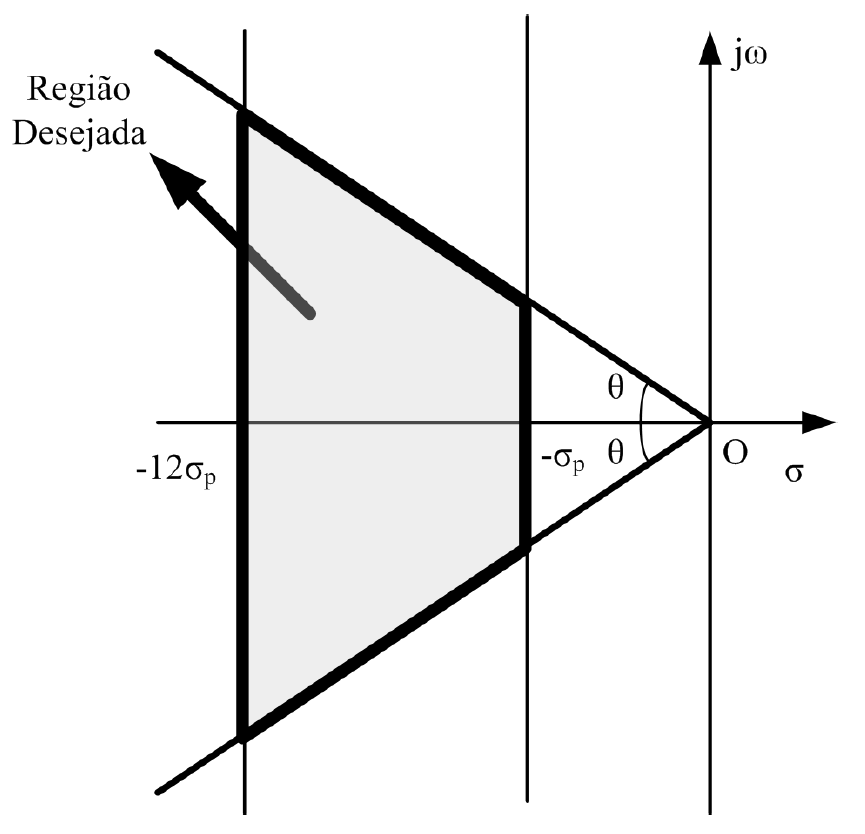
\includegraphics[width=7cm,height=5.25cm]{img/regiao_destabilidade.png}
    \caption{Região desejada de estabilidade, fonte \cite{CostaControleEolica}}
    \label{eq:dsta:regiao}
  \end{centering}
\end{figure}
\FloatBarrier

Em que $-\sigma_p$, $-\beta_p$ e $\theta$ são obtidas com os parâmetros deseja-dos em \eqref{eq:wnxi}, sendo que $\theta=\pi-\cos^{-1}(\xi)$. Considera-se um sistema ́e \( \mathcal{D}\)-estável quando as restrições \eqref{eq:dsta:lmis} e \eqref{eq:dsta:lmisaux} são satisfeitas. Segundo \cite{AguirreEncic}, o controle \( \mathcal{D}\)-alocação de polos resume-se em aplicar os conceitos de \( \mathcal{D}\)-estabilidade na busca de um ganho $K$ que satisfaça os autovalores do polinômio característico em malha fechada modelado no espaço de estados.
%    \section{Metodologia}
%        \subsection{Projeto de um controlador por realimentação de estados} 
A alocação dos autovalores $\lambda = \sigma \pm \omega_n.i$ é determinada a partir da aplicação dos valores encontrados nas equações   e 

\begin{align} \label{eq:autovalores_de_xi}
     \lambda = \omega_n * (-\xi \pm \sqrt{1-\xi^2}.i)
\end{align}
    
O ganho de realimentação para alocação de autovalores em malha fechada é computado através da equação de Lyapunov conforme descrito na seção   conforme exibido a seguir:
    
    \begin{equation*} 
    \begin{split}
        \mathbf{F} =
        \begin{bmatrix}
            -43.5923 &  47.1507 &       0       & 0 & \\ 
            -47.1507 & -43.5923 &       0 &       0 & \\
                   0 &        0 & -8.7185 &  9.4301 & \\
                   0 &        0 & -9.4301 & -8.7185 & \\
        \end{bmatrix}
    \end{split}
    \end{equation*} 
 
    \begin{equation*} 
    \begin{split}
        \mathbf{B} = B_u = 
        \begin{bmatrix}
            0 & \\
            -\frac{1}{m_s}&\\ \\
            0 & \\
            \frac{1}{m_u} \\
        \end{bmatrix};\ \
    \end{split}
    \begin{split}
    \mathbf{\bar{K}} =
        \begin{bmatrix}
        1&0&1&0&
        \end{bmatrix}
    \end{split}
    \end{equation*} 
    
    Resolvendo a equação de Lyapunov \ref{eq:lyapunov} para $T$ e substituindo a matriz T encontrada na equação \ref{eq:ganho} obtém-se os seguintes valores de ganhos de realimentação, valores arredondados na quarta casa decimal:
    
    \begin{center}
    \begin{tabular}{|c|c|}
        \hline
        Estado & Ganho\\
        \hline
        \hline
        $x_1$    & -18023.2837\\
        $x_2$    & -4567.6793\\
        $x_3$    & 13118.63414\\   
        $x_4$    & 2758.2869 \\
        \hline
    \end{tabular}
    \end{center}
    
\subsection{Simulação da resposta temporal do modelo linearizado em malha fechada com controlador por realimentação de estados} \label{sc:analise_resposta}
    
Abaixo seguem gráficos que ilustram a simulação temporal da resposta do sistema linearizado para excitação com entrada em "lombada" degrau de 0.1m:
  
\subsection{Simulação da resposta temporal do sistema em malha fechada considerando o sistema não linear original utilizando o controlador projetado para o sistema linear}
    
Abaixo seguem gráficos que ilustram a simulação temporal da resposta do sistema não linear comparada com a resposta do sistema linearizado para excitação com entrada em "lombada" degrau de 0.1m:

A observação dos gráficos da resposta temporal exibida nas figuras  traz a conclusão que, para este caso específico, a resposta temporal do sistema não linear em malha fechada com o controlador projetado para o sistema linearizado se mostrou muito semelhante a resposta temporal do sistema linear. Neste caso, contribuíram para isto a excitação com "lombada" em degrau pequena afastou pouco o sistema do ponto de equilíbrio, ao mesmo tempo que um controlador com um amortecimento relativamente alto, $\xi \simeq 0.6$, contribuiu para que a resposta transitória rica em frequências fosse rapidamente cancelada e apenas o comportamento em regime fosse exibido a maior parte do tempo.
    
Para comparação, é exibido a seguir a mesma simulação temporal para uma entrada com "lombada" em degrau unitário. Esta entrada excita mais frequências de ambos os sistema e podem revelar mais informações sobre as diferenças entre ambos os sistemas pois leva o sistema linearizado para uma condição de operação mais afastada do ponto de equilíbrio: 
    
A observação dos gráficos da resposta temporal exibida nas figuras demonstra que para uma entrada que desloque o sistema para uma região muito distante do ponto de equilíbrio utilizado para linearização pode causar uma grande diferença na resposta temporal do controle em malha fechada, inclusive podendo degradar significativamente o desempenho do controlador por realimentação de estados.  
        
\subsection{Simulação da resposta temporal em malha fechada com o controlador projetado para o sistema linearizado e considerando perturbação}
 
Abaixo seguem gráficos que ilustram a simulação temporal da resposta do sistema linearizado para excitação com perturbações em degraus aleatórios entre $\pm$ 5cm.

Para a análise da resposta dinâmica do sistema controlado permanecem válidas as mesmas considerações apresentadas na seção \ref{sc:analise_resposta}


    \section{Resultados}
        \subsection{Modelo numérico do sistema de suspensão ativa}
Com base nas matrizes A e B do sistema linearizado obtidas em \ref{ed:linsys:ax} e \ref{ed:linsys:BuBw} e nos parâmetros na tabela \ref{tb:parametros} do Apêndice, obtemos os seguintes valores numéricos do sistema LTI que será utilizado no benchmark deste trabalho, considerou-se que o sistema é um LPV com incerteza paramétrica $\delta$ na massa do veiculo, podendo variar em $\pm 100 kg$ ao redor do valor nominal do modelo de dependendo do carregamento do veiculo:
%\ms, \mus, \bls, \bnls, \bys, \kls, \knls, \kt

\begin{equation}\label{ed:linsys:ALPV}
    \begin{split}
        \mathbf{A} =
        \begin{bmatrix}
            0 & 1 & 0 & 0 & \\            
            -\frac{\kls}{\ms+\delta}&-\frac{\bls}{\ms+\delta}&\frac{\kls}{\ms+\delta}&\frac{\bls}{\ms+\delta} &\\ \  
            0 & 0 & 0 & 1 & \\
            \frac{\kls}{\mus}&\frac{\bls}{\mus}&-\frac{(6925.1077\cdot10^{3})}{\mus}&-\frac{\bls}{\mus} &\\
        \end{bmatrix}
    \end{split}
\end{equation}

\begin{equation}\label{ed:linsys:BLPV}
    \begin{split}
        \mathbf{B_u} = 
        \begin{bmatrix}
            0 & \\            
            -\frac{1}{\ms+\delta}&\\ \\  
            0 & \\
            \frac{1}{\mus}&\\
        \end{bmatrix};
    \end{split}
    \begin{split}
        \mathbf{B_w} = 
        \begin{bmatrix}
            0 & \\            
            0 &\\ \\  
            0 & \\
            \frac{\kt}{\mus}& \\
        \end{bmatrix}
    \end{split}
\end{equation}

Para a matriz $\mathbf{C}$ consideraremos ser possível a leitura de todos os estados do sistema, e para as matrizes $D_u$ e $D_w$, consideramos que não há termo de transmissão direta das entradas, como exibido a seguir:

\begin{equation} \label{eq:matriz_c}
    \begin{split}
        \mathbf{C}=
    \end{split}
    \begin{bmatrix}
        1&0&0&0&\\
        0&1&0&0&\\
        0&0&1&0&\\
        0&0&0&1&\\
    \end{bmatrix};\ \
    \begin{split}
        \mathbf{D_u} = 0
    \end{split};\ \
    \begin{split}
        \mathbf{D_w} = 0
    \end{split};\ \ 
\end{equation}

\subsection{Especificação da região de \( \mathcal{D}\)-estabilidade desejada}
Deseja-se um valor de Máximo overshoot percentual de $M_O \leq 10$ \% e Tempo de acomodação para a faixa de tolerância de 2 \% $T_S \leq 0.5$ s. 
Dada a equação para o cálculo da taxa de amortecimento para um valor de máximo overshoot dado, obtém-se o seguinte valor objetivo para $\xi$:

\begin{equation*}
    \xi=-\frac{ln\left(0.1\right)}{\sqrt{\pi^2+ln^2(0.1)}}=0.5912
\end{equation*}

Dada a equação para o cálculo da $\omega_n$ objetivo para um tempo de assentamento dado, obtém-se o seguinte valor objetivo para $\omega_n$:

\begin{equation*}
    \omega_n=-\frac{ln\left( 0.02*\sqrt{1-0.5912} \right)}{0.5*0.5912}=13.5328
\end{equation*}

Para $\xi=0.5912$ e $\omega_n=13.5328$ os parâmetros $\sigma_p$ e $\theta$ são obtidos como se segue

\begin{equation}\label{ed:dstab:params}
    \begin{split}
       \sigma_p=-\omega_n=-13.5328\ \ rad\cdot s^{-1}\\
       \theta=\pi-\cos{(\xi)}^{-1}=0.9383\ \ rad\\    
    \end{split}
\end{equation}

Apenas para limitar a região de \( \mathcal{D}\)-estabilidade desejada, tomaremos o limite a esquerda como sendo $20\cdot\sigma_p$. A região de \( \mathcal{D}\)-estabilidade definida para acomodação do sistema é exibida na figura \ref{eq:dsta:regiaodef} a seguir:

\FloatBarrier
\begin{figure}[htbp] 
  \begin{centering}
    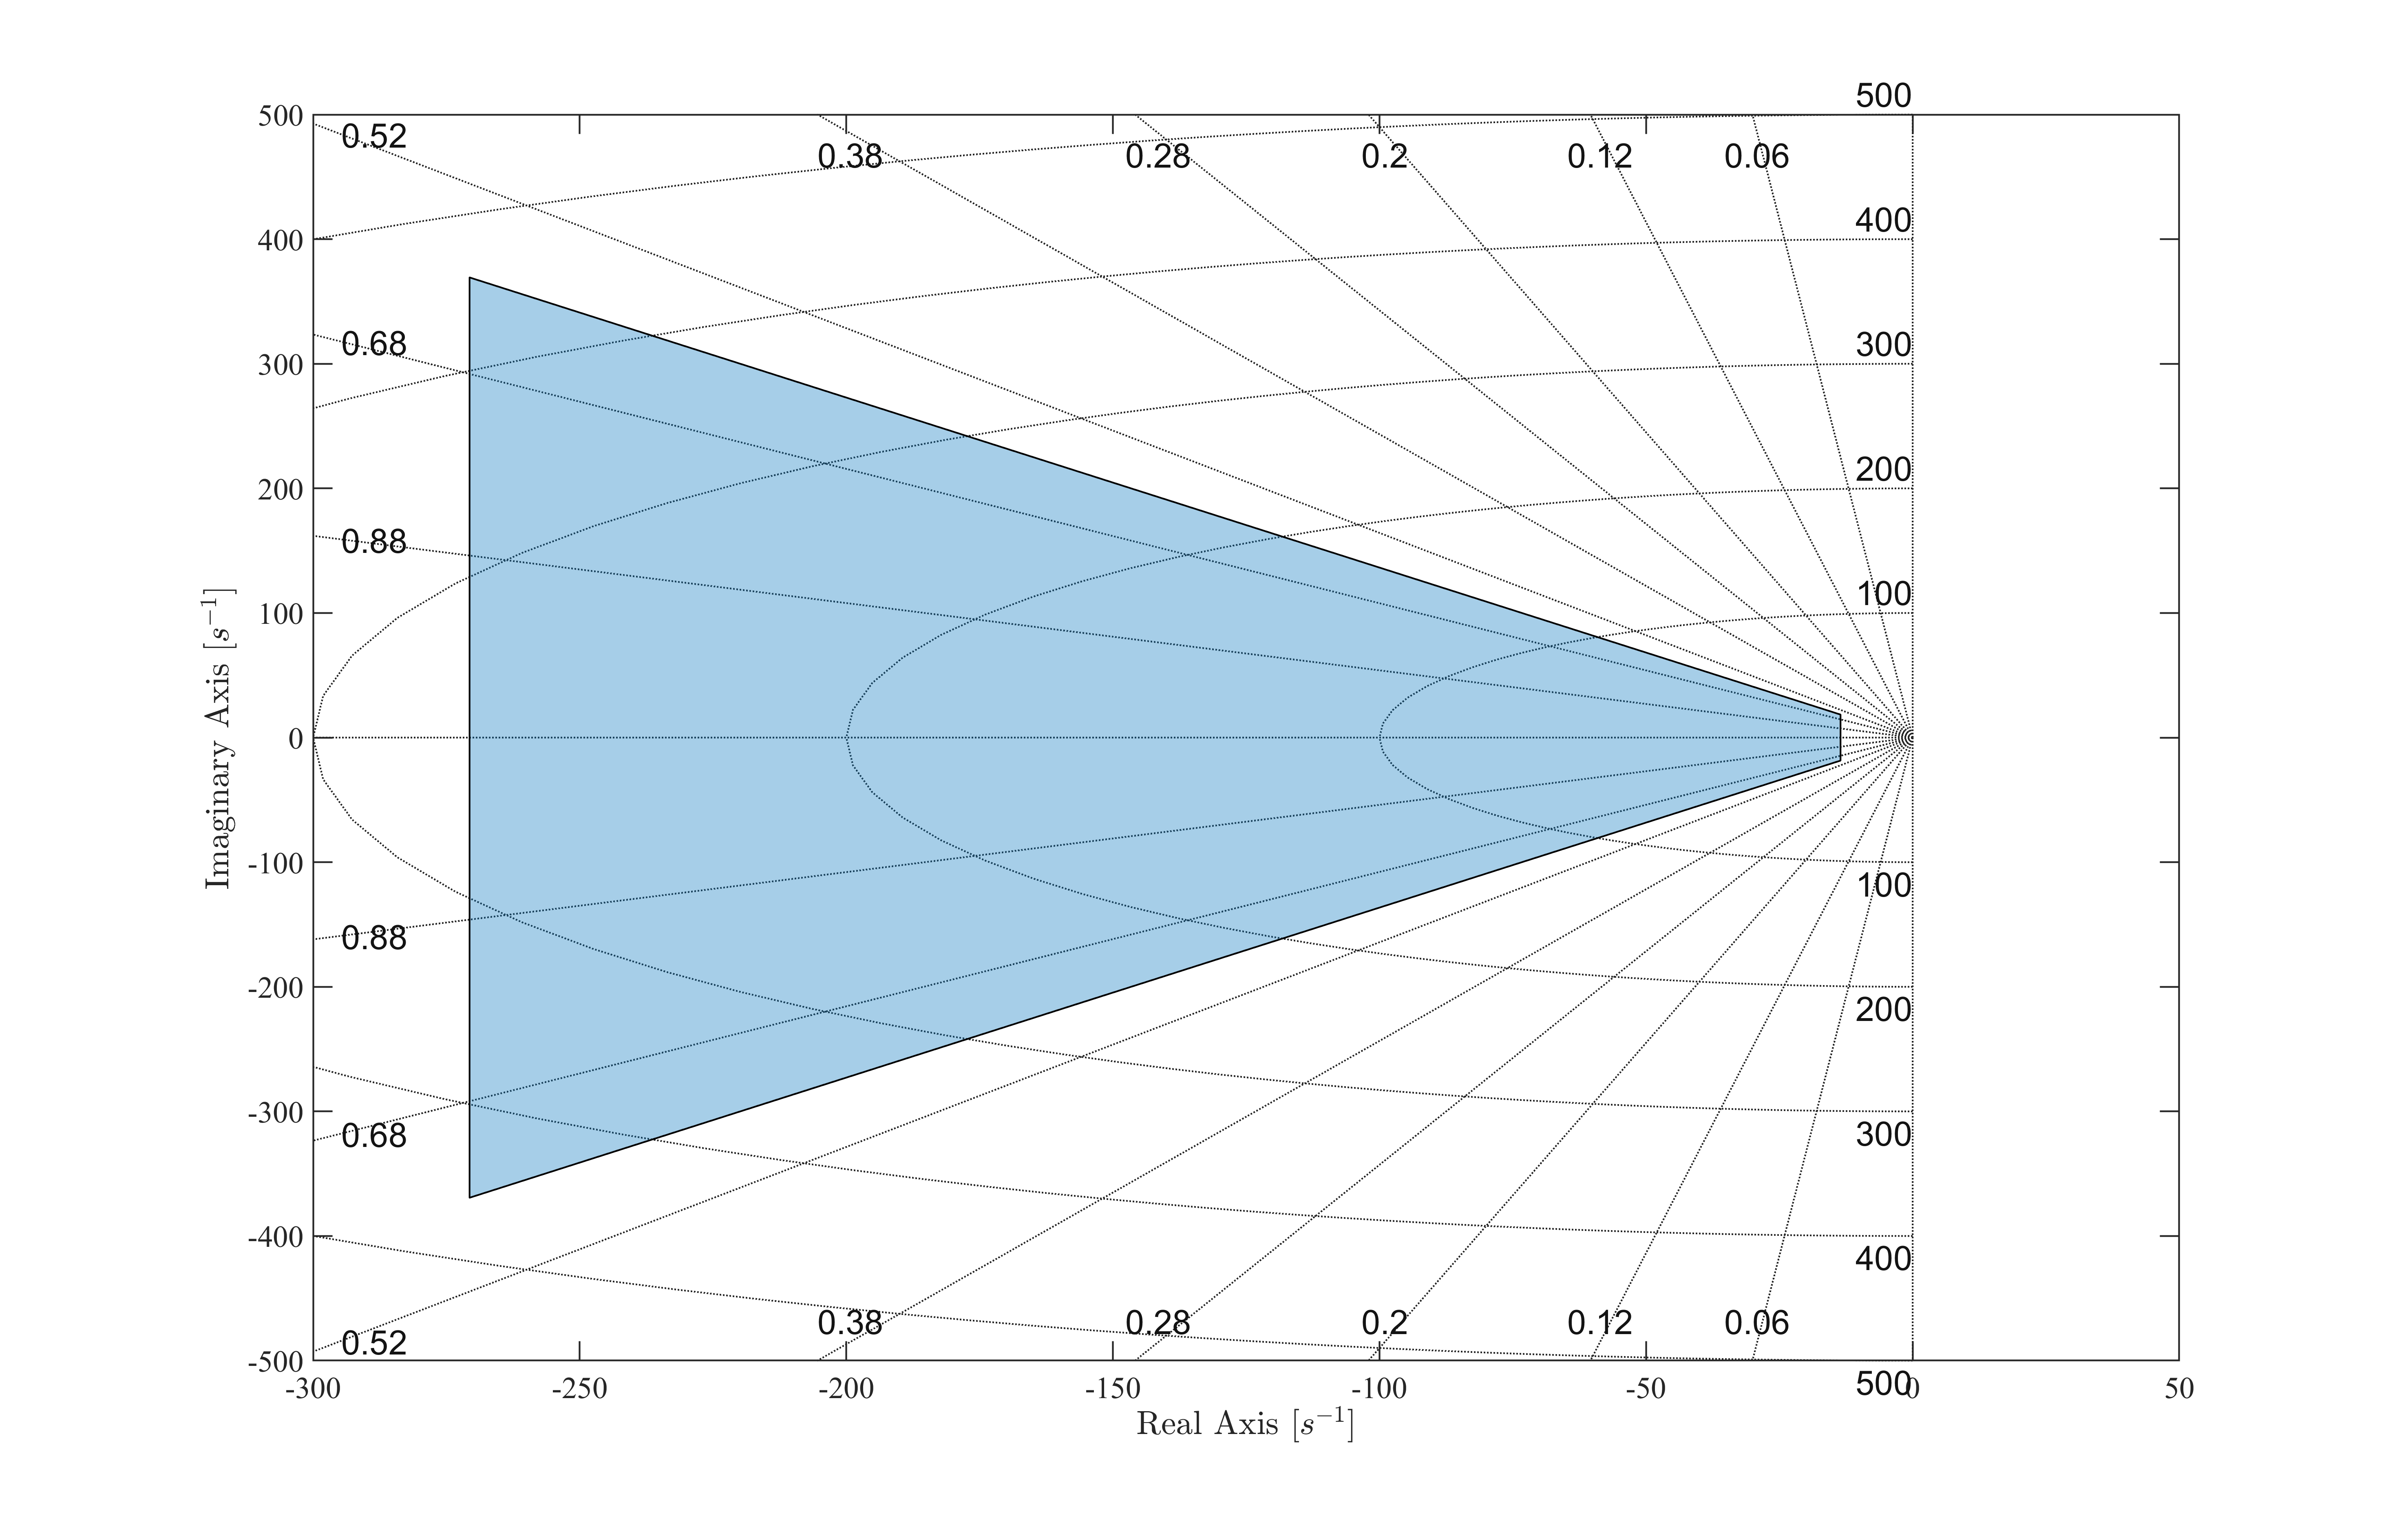
\includegraphics[width=8cm,height=6cm]{img/regiao_d_estabilidade.png}
    \caption{Região definida de estabilidade}
    \label{eq:dsta:regiaodef}
  \end{centering}
\end{figure}
\FloatBarrier

\subsection{Controlador Robusto por realimentação de estados com \( \mathcal{D}\)-estabilidade garantida}
Considerando o sistema no espaço de estados apresentado em \eqref{eq:dsta:linsys} com incerteza paramétrica nas matrizes $A$ e $B$, cujos valores são apresentados em \eqref{ed:linsys:ALPV} e \eqref{ed:linsys:BLPV}, em que o parâmetro $\delta$ representa a incerteza do modelo associada a massa do veiculo de $\pm100kg$. A síntese do  controlador  robusto ́e  realizada  pela  resolução das LMIs \eqref{eq:dsta:lmis} e \eqref{eq:dsta:lmisaux} para os parâmetros da região de \( \mathcal{D}\)-estabilidade definidos em \eqref{ed:dstab:params}. Os ganhos obtidos do procedimento de otimização são exibidos abaixo com precisão de 4 casas decimais:

\begin{equation*} \label{eq:ganhoscontrolador}
    K^'=
    \begin{bmatrix}
        -514929.0792&\\	
        -51637.9194&\\	
        791876.7347&\\
        2492.4857&\\
    \end{bmatrix}
\end{equation*}

Calculou-se a localização dos autovalores do sistema para os valores de $\sigma = -100, -90, \dots, 90, 100$ e os resultados são exibidos na figura abaixo, com o sistema em malha aberta e malha fechada.
\FloatBarrier
\begin{figure}[htbp]
    \begin{centering}
    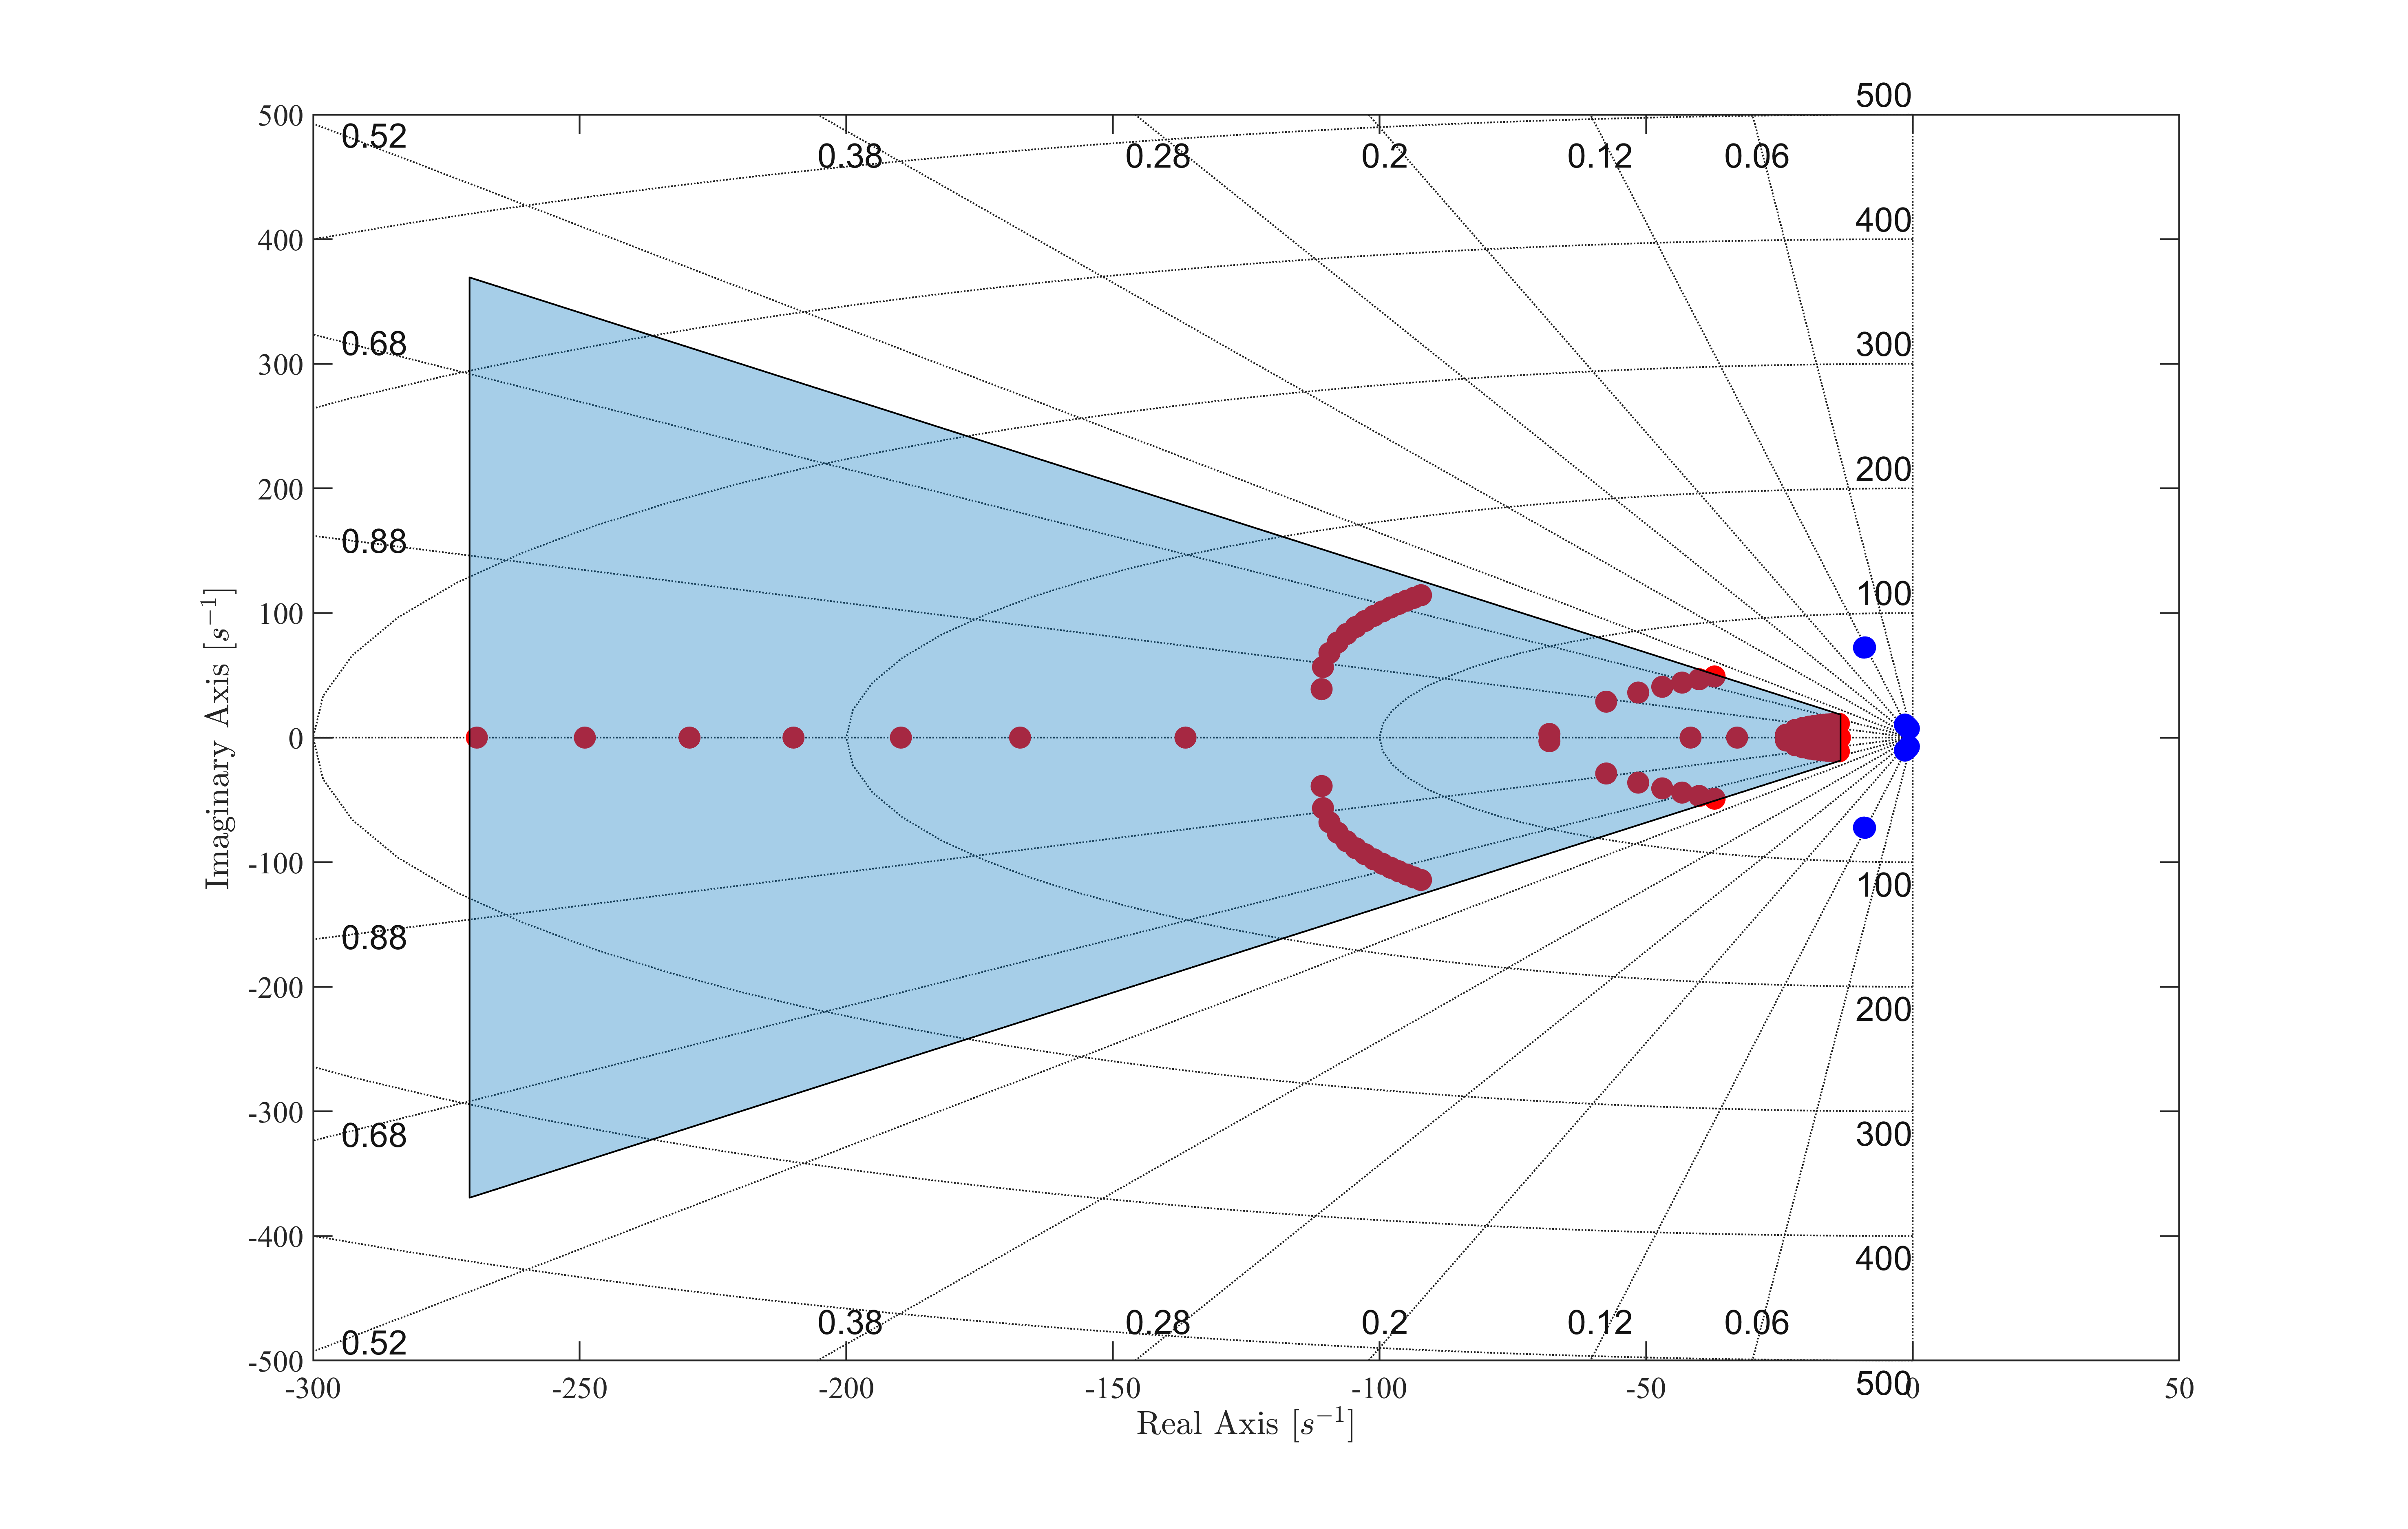
\includegraphics[width=8cm]{img/regiao_d_estabilidade_autoval.png}
    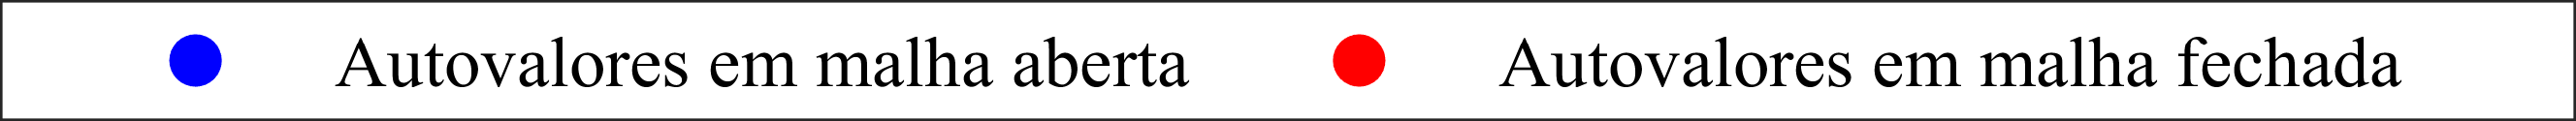
\includegraphics[width=6cm]{img/regiao_d_estabilidade_autoval_leg.png}
    \caption{Autovalores do sistema}
    \label{fig:regiao_d_estabilidade_autoval_leg}
    \end{centering}
\end{figure}
\FloatBarrier
    \section{Conclusão}
        O principal objetivo do trabalho foi analisar o efeito do uso de observadores de entradas desconhecidas robustos na síntese de um sistema de controle por realimentação de estados baseado em observador para um sistema de suspensão veicular, linear, invariante no tempo com dependência paramétrica e incertezas politópicas. Foram propostas condições para estimar os estados do sistema na presença de distúrbios desconhecidos.  
Em seguida foi projetado um controlador de realimentação de estados baseados nos estados observados com \( \mathcal{D}\)-estabilidade e requisitos de desempenho temporal garantidos. Os resultados apresentados mostram que a metodologia não foi eficaz para estimar os estados não medidos, mesmo napresença de entradas desconhecidas, e utilizar os estados estimados para o controle dossistemas estudados
    \bibliography{references,manual}    
    \appendix
        \section{\\Lista de siglas e abreviações}
    \begin{itemize} 
        \item [LTI] Linear e invariante no tempo.
        \item [UIO] Observador de entradas desconhecidas.
        \item [SISO] Single Input, Single Output.
        \item [LMI] Desigualdade Matricial Linear.
        \item [LPV] Sistemas lineares com dependência paramétrica.
        %\item [$m_s$] Massa suspensa.
%        \item [$m_u$] Massa não suspensa.
 %       \item [$b_s$] Coeficiente de amortecimento do amortecedor passivo. 
   %     \item [$k_s$] Coeficiente de elasticidade do feixe de molas da suspensão.
   %     \item [$k_t$] Coeficiente de elasticidade do pneu.
     %   \item [$x_r$] Deslocamento vertical da pista.
 %       \item [$x_w$] Deslocamento vertical da roda.
 %       \item [$x_c$] Deslocamento vertical da carroceria.
     %   \item [$\dot{x}_w$] Velocidade vertical da roda.
  %      \item [$\dot{x}_c$] Velocidade vertical da carroceria.
  %      \item [$F$] Força aplicada pelo amortecedor ativo ou semi-ativo.
 %       \item [$k^{l}_{s}$] Coeficiente de elasticidade do termo linear no modelo %não linear do feixe de olas da suspensão.
 %       \item [$k^{nl}_{s}$] Coeficiente de elasticidade do termo não linear no %modelo não linear do feixe de molas da suspensão.
 %       \item [$b^{l}_{s}$] Coeficiente de amortecimento do termo da faixa de %operação linear do amortecedor.
  %     \item [$b^{l}_{s}$] Coeficiente de amortecimento do termo da faixa de %operação não linear do amortecedor.
   %     \item [$b^{y}_{s}$] Coeficiente que representa a característica  de %comportamento assimétrico do amortecedor.
    \end{itemize}
\section{}\listoffigures   
\end{document}